\section{Fluxional execution model} \label{section:model}

The compiler we present in section \ref{section:compiler} focus on web applications that tend to follow the functional paradigm while keeping a global memory.
Such applications are built using functions that are executed sequentially to assure the exclusivity of access on the global memory.
This is a serious performance issue, as it avoids to leverage the parallelism of modern architectures.

We present in this section a different execution model that isolate the memory accessible to some functions.
This approach allows to execute these functions in parallel, hence, to benefit of the performance improvements of this parallelism.
This execution model is close to the actor model, as the function are executed on autonomous execution unit with their own isolated memory, communicating by messages.
Because we focus on real-time web applications, we insist on the streaming nature of these communications.
The execution units exchange streams of messages, that correspond with the input stream of requests of the web application.

\subsection{Fluxions and workers}

The fluxional execution model manages and invokes autonomous execution units named fluxion $\bnfpn{flx}$.
A fluxion is composed of a unique name $\bnfpn{id}$, a processing function $\bnfpn{fn}$, and a persisted memory called a \textit{context} $\bnfpn{ctx}$.
Its function $\bnfpn{fn}$ consumes an input stream $\bnfpn{stream}$ and generates one or more outputs streams to other fluxions $\bnfpn{dest}$.
The \textit{context} persists the state on which a fluxion relies between two message receptions.
At a message reception, the fluxion modifies its \textit{context}, and sends back messages to downstream fluxions.
A message is composed of the recipient fluxions' names and a body.

Fluxions are executed on workers.
A worker is an event-loop and an isolated heap ; it is a \textit{Node.js} instance.
The context of a fluxion is lexically isolated.
It has a distinct lexical scope containing variables not shared with any other fluxion.
However, fluxions on the same worker share the same event-loop, and the same heap ; they can send references to each over.
Fluxions on different workers have different event-loops and heaps ; their communications are serialized, so it is useless to send heap references.
Fluxions are the stages in a pipeline architecture.
The streams of messages between fluxions are carried by the messaging system.

The event-loop assures the exclusivity of operations on the heap.
Only one fluxion is executed at once on a worker.
Consequently, the more fluxions share states, the less time fraction each fluxion has for its execution.
If a fluxion has its own exclusive state, it can be parallelized.

We represent here the syntax of a high-level language to represent a program in the fluxionnal form.
It is the target for our compiler.
\begin{bnf*}
  \bnfprod{program}    {\bnfpn{flx} \bnfor \bnfpn{flx} \bnfsp \bnftd{eol} \bnfsp \bnfpn{program}}\\
  \bnfprod{flx}        {\bnfts{\texttt{flx}} \bnfsp \bnfpn{id} \bnfsp \bnfpn{ctx} \bnfsp \bnfpn{worker} \bnfsp \bnftd{eol} \bnfsp \bnfpn{streams} \bnfsp \bnftd{eol} \bnfsp \bnfpn{fn}}\\
  \bnfprod{worker}     {\bnfts{\texttt{on}} \bnfsp \bnfpn{id} \bnfor \bnftd{empty string}}\\
  \bnfprod{streams}    {\bnfts{\texttt{null}} \bnfor \bnfpn{stream} \bnfor \bnfpn{stream} \bnfsp \bnftd{eol} \bnfsp \bnfpn{streams}}\\
  \bnfprod{stream}     {\bnfpn{op} \bnfsp \bnfpn{dest} \bnfsp [\bnfpn{msg}]}\\
  \bnfprod{dest}       {\bnfpn{list}}\\
  \bnfprod{ctx}        {\bnfts{\texttt{\{}} \bnfpn{list} \bnfts{\texttt{\}}}}\\
  \bnfprod{msg}        {\bnfts{\texttt{[}} \bnfpn{list} \bnfts{\texttt{]}}}\\
  \bnfprod{list}       {\bnfpn{id} \bnfor \bnfpn{id} \bnfsp \bnfts{,} \bnfsp \bnfpn{list}}\\
  \bnfprod{op}         {\bnfts{\texttt{>}\texttt{>}} \bnfor \bnfts{\texttt{-}\texttt{>}}}\\
  \bnfprod{id}         {\bnftd{Javascript identifier}}\\
  \bnfprod{fn}         {\bnftd{Javascript and stream syntax}}\\
\end{bnf*}
\vspace{-2.5\baselineskip}


\subsection{Messaging system}

In a distributed approach, the messages between fluxions would be carried over a distributed message broker.
However this execution model is only a simulation of a distributed execution environement.
We simplify the distributed message broker with a master message queue to centralize communication between workers, though, each worker has its own local message queue.
% The messaging system is the core of the execution model.
% It carries messages and invokes fluxions at reception.
The messaging system sends messages to the worker hosting the destination fluxion.
Locally, the master worker hosts fluxions that need access to the external network or the global memory.
% Using a message queue allows to execute multiple processing chains fairly and concurrently, without difference in scheduling local messages, or network messages.

The execution cycle of a fluxional application is illustrated in figure \ref{fig:MesSys}.
Circles represent registered fluxions.
The fluxion \textit{reply} has a context containing the variable \texttt{count}.
The plain arrows represent the actual message paths in the messaging system, while the dashed lines between fluxions represent the message streams as seen in the fluxionnal application.
The streams between workers are serialized.

\begin{figure}[h!]
  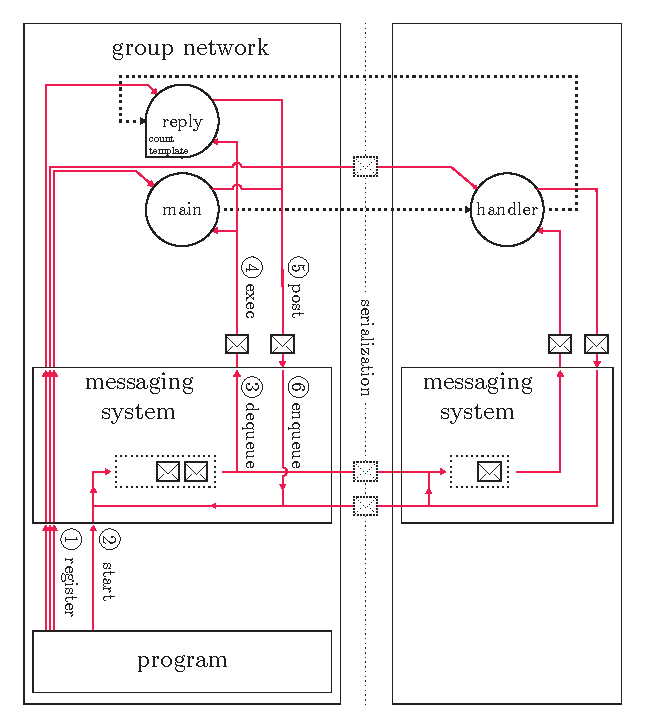
\includegraphics[width=\linewidth]{ressources/schema-message.pdf}
  \caption{The fluxionnal execution model in details}
  \label{fig:MesSys}
\end{figure}

The messaging system carries messages based on the names of the recipient fluxions.
If two fluxions share the same name, it would lead to a conflicting situation for the messaging system.
Every fluxion needs to be registered with a unique name.
This registration associates a processing function with a unique name and an initial \textit{context}.
The registration is done by calling \texttt{register(<name>, <fn>, <context>)}, \circled{1}.
% A fluxion can dynamically register other fluxions

When a new request is received, a \texttt{start} message triggers the flow using the function \texttt{start(<msg>)}, \circled{2}.
This first message represent the incoming of a request from a user.
The system dequeues this message and dispatch it to the destination fluxion, \textit{handler}, \circled{3} and \circled{4}.
The fluxion \textit{handler} sends back a message using the function \texttt{post(<msg>)}, \circled{5}, to be enqueued in the centralized message queue, \circled{6}.
The system loops through steps \circled{3} and \circled{4} until the queue is empty.
This cycle starts again for each new incoming request causing a \texttt{start} message.

% Algorithms \ref{alg:parcours} and \ref{alg:traitement} describe the behavior of the messaging system after the \texttt{start} function invocation.

% \begin{algorithm}
% \caption{Message queue walking algorithm}
% \label{alg:parcours}
% \begin{algorithmic}
% \Function{loopMessage}{\null}
% \While{$msg$ \textbf{presents in} $msgQueue$}
% \State $msg \gets$ \Call{dequeue}{\null} \Comment{\circled{3}}
% \State \Call{ProcessMsg}{$msg$}
% \EndWhile
% \EndFunction
% \end{algorithmic}
% \end{algorithm}

% \begin{algorithm}
% \caption{Message processing algorithm}
% \label{alg:traitement}
% \begin{algorithmic}
% \Function{processMsg}{$msg$}
% \For{$dest$ \textbf{in} $msg.dest$}
% \State $worker \gets lookup(dest)$
% \State \Call{worker.send}{$fluxion, msg.body$} \Comment{\circled{4}}
% % \State $message \gets$ \Call{exec}{$fluxion, msg.body$} \Comment{\circled{4} \& \circled{5}}
% % \State \Call{enqueue}{$message$} \Comment{\circled{6}}
% \EndFor
% \EndFunction
% \end{algorithmic}
% \end{algorithm}

\subsection{Service example}

To illustrate the fluxional execution model, and the compiler we present an example of a simple web application.
This application reads the file containing its own source code, and sends it back along with a request counter.

The original source code of this application is available on github\cite{flx-example}, and in listing \ref{lst:source}.
In this source code, some points are worth noticing.
The \texttt{handler} function, line 5 to 11, receives the input stream of request.
It is the first function we execute in an isolated fluxion.
The \texttt{count} variable at line 3 increments the request counter.
This object needs to be persisted in the fluxion \textit{execution context}.
The \texttt{app.get} and \texttt{app.send} methods, respectively line 5 and 9, interface the application with the clients.
The processing chain of functions occurs between these two functions : $\texttt{get} \twoheadrightarrow \texttt{handler} \to \texttt{readFile} \to \texttt{reply} \to \texttt{send}$.

\begin{code}[js,
  caption={Simple web application that replies to every request with its own source code and a counter},
  label={lst:source}]
var app = require('express')(),
    fs = require('fs'),
    count = 0;

app.get('/', function handler(req, res){
  fs.readFile(__filename, function reply(err, data) {
    count += 1;
    res.send(err || template(count, data));
  });
});

app.listen(8080);
\end{code}

This application is transformed manually into the high-level fluxionnal language in listing \ref{lst:fluxional}, and illustred in Figure \ref{fig:MesSys}.
We expect a similar result with the compiler described in section \ref{section:compiler}.
% Horizontal dashed lines show virtual transmission of messages between fluxions although they all go through the messaging system.

% \begin{figure}[h!]
%   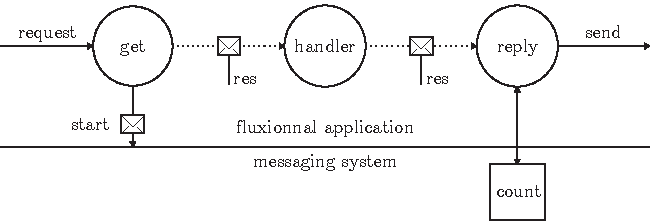
\includegraphics[width=\linewidth]{ressources/flux.pdf}
%   \caption{Fluxions chain manually extracted from the example application}
%   \label{fig:fluxions}
% \end{figure}

\begin{code}[flx, caption={Manual transformation of the example application in our high-level fluxional language},label={lst:fluxional}]
flx get
>> handler [res]
  var app = require('express')(),
      fs = require('fs'),
      count = 0;

  app.get('/', >> handler); //@\label{lst:fluxional-streamtohandler}@
  app.listen(8080);

flx handler on worker
-> reply [res]
  function handler(req, res) {
    fs.readFile(__filename, -> reply); //@\label{lst:fluxional-readfile}@
  }

flx reply {count, template}
-> null
  function reply(error, data) {
    count += 1; //@\label{lst:fluxional-counter}@
    res.send(err || template(count, data)); //@\label{lst:fluxional-ressend}@
  }
\end{code}

The application is organized as follow :
\begin{itemize}
  \item The \texttt{get} fluxion is the \textit{root} fluxion.
  It initializes the application to listen for user requests by calling \texttt{app.get}.
  Every request is forwarded on the stream to the \texttt{handler} fluxion, line \ref{lst:fluxional-streamtohandler}.
  \item The \texttt{handler} fluxion reads the file containing the source code of the application, and forwards the result to the \texttt{reply} fluxion, line \ref{lst:fluxional-readfile}.
  \item The \texttt{reply} fluxion increments the counter, line \ref{lst:fluxional-counter}, formats the reply, and sends it back to the user using the function \texttt{res.send}, line \ref{lst:fluxional-ressend}.
\end{itemize}

Our goal, as described in the introduction, is not to propose a new programming paradigm with this high-level language but to automate the architecture shift with a compiler.
We present this compiler in the next section.